\subsection{Meta}

La principal jerarquía de elementos de comportamiento y estructura del lenguaje ArchiMate se presenta en la tabla 3.1. Define estos elementos de forma genérica e independiente de la capa. Nótese que la mayoría de estos elementos (las cajas blancas) son elementos abstractos del metamodelo; es decir, no están instanciados en los modelos sino que sólo sirven para estructurar el metamodelo.  La notación presentada es, por lo tanto, la forma genérica en que se representan las especializaciones de estos elementos (es decir, los elementos de las diferentes capas de la arquitectura). Además de describir  los elementos concretos (los recuadros grises), que pueden utilizarse para modelar la Arquitectura de la Empresa a nivel estratégico.

\newpage
\subsubsection{Elementos de la Estructura}
	\begin{table}[h!]
	\begin{tabular}{| m{7em} | m{7cm} | m{3cm} |}
		\hline
		Concepto & Descripción & Representación \\
		
		\hline
		Motivación
		& 
		Un elemento de motivación representa el contexto o la motivación detrás de la  arquitectura de la empresa
		& 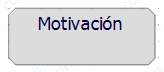
\includegraphics[width=0.8\linewidth, height=0.05\textheight]{imgs/conceptos/meta/Motivacion}
		\\
		
		\hline
		Estructura 
		& 
		Elementos de estructura son equivalentes sinónimos, se subdividen  en estructuras activas ,                              estructuras activas internas,  estructuras activas externas y estructuras pasivas
		& 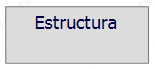
\includegraphics[width=0.8\linewidth, height=0.05\textheight]{imgs/conceptos/meta/Estructura}
		\\
		
		\hline
		Estructura activa  
		& 
		Estructuras que pueden tener un comportamiento
		& 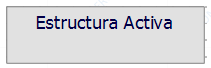
\includegraphics[width=0.8\linewidth, height=0.05\textheight]{imgs/conceptos/meta/EstructuraActiva}
		\\  
		
		\hline
		Estructura activa externa  
		& 
		Llamado interfase representa un punto de acceso donde uno o mas servicios son prestados al ambiente  
		&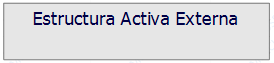
\includegraphics[width=0.8\linewidth, height=0.05\textheight]{imgs/conceptos/meta/EstructuraActivaExterna}
		\\
		
		\hline
		Estructura activa interna
		& 
		Es un elemento que representa una entidad que es capaz de mostrar comportamiento
		& 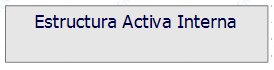
\includegraphics[width=0.8\linewidth, height=0.05\textheight]{imgs/conceptos/meta/EstructuraActivaInterna.PNG}
		\\
		
		\hline
		Estructura pasiva
		& 
		Es un elemento que representa una entidad sobre la cual se realiza un comportamiento
		& 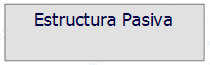
\includegraphics[width=0.8\linewidth, height=0.05\textheight]{imgs/conceptos/meta/EstructuraPasiva.PNG}
		\\
		
		\hline
		Interfase
		& 
		Representa un punto de acceso donde uno o mas servicios son puestos en el ambiente.
		& 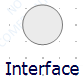
\includegraphics[width=0.8\linewidth, height=0.05\textheight]{imgs/conceptos/meta/Interface.PNG}
		\\
		
		\hline
		
		Comportamiento
		& 
		Es un elemento que equivale a un verbo se  subdivide en evento ,comportamiento interno, proceso , función, interacción, comportamiento externo y servicio.
		& 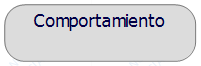
\includegraphics[width=0.8\linewidth, height=0.05\textheight]{imgs/conceptos/meta/Comportamiento.PNG}
		\\
		
		\hline
		Evento
		&
		Representa un cambio de estado 
		& 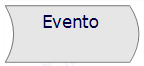
\includegraphics[width=0.8\linewidth, height=0.05\textheight]{imgs/conceptos/meta/Evento.PNG}
		\\
		
		\hline
		Elemento de comportamiento interno 
		& 
		Representa una o mas unidades de actividades que pueden ser realizadas por uno o mas elementos de estructura activa
		& 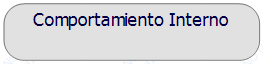
\includegraphics[width=0.8\linewidth, height=0.05\textheight]{imgs/conceptos/meta/ComportamientoInterno.PNG}
		\\	\hline
	\end{tabular}
	%\caption{}
	\label{tab:concepts}
\end{table}

\newpage
\begin{table}[h!]
\begin{center}
	\begin{tabular}{| m{6em} | m{7cm} | m{3cm} |}
		\hline
		Concepto & Descripción & Representación \\ 
		
		\hline
		Servicio
		&
		Un servicio es un comportamiento del sistema proveedor  visible  externamente 
		&
		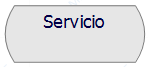
\includegraphics[width=0.8\linewidth, height=0.05\textheight]{imgs/conceptos/meta/Servicio.PNG}
		\\
		
		\hline
		Función
		& 
		Representa una colección de comportamientos, basado en una colección de criterios específicos, tales como fuente requerida, competencias o localización   
		& 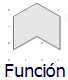
\includegraphics[width=0.8\linewidth, height=0.05\textheight]{imgs/conceptos/meta/Funcion.PNG}
		\\
		
		\hline
		Proceso
		& 
		Representa una secuencia de comportamientos que consiguen un resultado especifico
		& 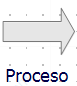
\includegraphics[width=0.8\linewidth, height=0.05\textheight]{imgs/conceptos/meta/Proceso.PNG}
		\\
		
		\hline
		Interacción  
		& 
		Representa una unidad de comportamientos que deben ser realizados por dos o mas elementos de estructura activa interna , ya sea a través de una asignación directa o agregados en una colaboración 
		& 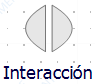
\includegraphics[width=0.8\linewidth, height=0.05\textheight]{imgs/conceptos/meta/Interaccion.PNG}
		\\
		
		\hline
		Colaboración  
		& 
		Representa un acuerdo entre dos o mas elementos estructuras activas internas, trabajan juntos para realizar algún comportamiento colectivo   
		& 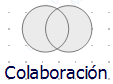
\includegraphics[width=0.8\linewidth, height=0.05\textheight]{imgs/conceptos/meta/Colaboracion.PNG}
		\\
		
		\hline
		Elemento de comportamiento externo
		& 
		Representa un comportamiento explicito que es visible en el exterior  
		& 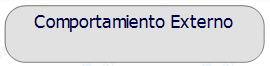
\includegraphics[width=0.8\linewidth, height=0.05\textheight]{imgs/conceptos/meta/ComportamientoExterno.PNG}
		\\
		
		\hline
		
		Elementos compuestos 
		&
		Son elementos que se basan en aspectos de otras capas del lenguaje   
		&
		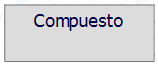
\includegraphics[width=0.8\linewidth, height=0.05\textheight]{imgs/conceptos/meta/Compuesto.PNG}
		\\
		
		\hline
	\end{tabular}
	\caption{Conceptos capa meta}
	\label{tab:concepts}
\end{center}
\end{table}